% !TeX program = xelatex
\documentclass[11pt, letterpaper]{article}
\title{MTH500 Assignment 1}
\author{Mustafif Khan}
\date{\today}
%%%%%%%%%%%%%%%%%%%%%%%%%%%%%%%%%%%%%%%%%
% Lachaise Assignment
% Structure Specification File
% Version 1.0 (26/6/2018)
%
% This template originates from:
% http://www.LaTeXTemplates.com
%
% Authors:
% Marion Lachaise & François Févotte
% Vel (vel@LaTeXTemplates.com)
%
% License:
% CC BY-NC-SA 3.0 (http://creativecommons.org/licenses/by-nc-sa/3.0/)
%
%%%%%%%%%%%%%%%%%%%%%%%%%%%%%%%%%%%%%%%%%
%----------------------------------------------------------------------------------------
%	PACKAGES AND OTHER DOCUMENT CONFIGURATIONS
%----------------------------------------------------------------------------------------
\usepackage{amsmath,amsfonts,stmaryrd,amssymb} % Math packages
\usepackage{enumerate} % Custom item numbers for enumerations
\usepackage[ruled]{algorithm2e} % Algorithms
\usepackage[framemethod=tikz]{mdframed} % Allows defining custom boxed/framed environments
\usepackage{listings} % File listings, with syntax highlighting
\lstset{
	basicstyle=\ttfamily, % Typeset listings in monospace font
}
%----------------------------------------------------------------------------------------
%	DOCUMENT MARGINS
%----------------------------------------------------------------------------------------
\usepackage{geometry} % Required for adjusting page dimensions and margins
\geometry{
	top=2.5cm, % Top margin
	bottom=3cm, % Bottom margin
	left=2.5cm, % Left margin
	right=2.5cm, % Right margin
	headheight=14pt, % Header height
	footskip=1.5cm, % Space from the bottom margin to the baseline of the footer
	headsep=1.2cm, % Space from the top margin to the baseline of the header
	%showframe, % Uncomment to show how the type block is set on the page
}
\usepackage{xcolor}

\definecolor{codegreen}{rgb}{0,0.6,0}
\definecolor{codegray}{rgb}{0.5,0.5,0.5}
\definecolor{codepurple}{rgb}{0.58,0,0.82}
\definecolor{backcolour}{rgb}{0.95,0.95,0.92}

\lstdefinestyle{mystyle}{
    commentstyle=\color{codegreen},
    keywordstyle=\color{blue},
    numberstyle=\tiny\color{codegray},
    stringstyle=\color{codepurple},
	basicstyle=\ttfamily\scriptsize,
	breakatwhitespace=false,
    breaklines=true,
    captionpos=b,
    keepspaces=true,
    showspaces=false,
    showstringspaces=false,
    showtabs=false,
    tabsize=4
}

\lstset{style=mystyle}
%----------------------------------------------------------------------------------------
%	FONTS
%----------------------------------------------------------------------------------------
\usepackage[utf8]{inputenc} % Required for inputting international characters
\usepackage[T1]{fontenc} % Output font encoding for international characters
\usepackage{XCharter} % Use the XCharter fonts
%----------------------------------------------------------------------------------------
%	COMMAND LINE ENVIRONMENT
%----------------------------------------------------------------------------------------
% Usage:
% \begin{commandline}
%	\begin{verbatim}
%		$ ls
%
%		Applications	Desktop	...
%	\end{verbatim}
% \end{commandline}
\mdfdefinestyle{commandline}{
	leftmargin=10pt,
	rightmargin=10pt,
	innerleftmargin=15pt,
	middlelinecolor=black!50!white,
	middlelinewidth=2pt,
	frametitlerule=false,
	backgroundcolor=black!5!white,
	frametitle={Command Line},
	frametitlefont={\normalfont\sffamily\color{white}\hspace{-1em}},
	frametitlebackgroundcolor=black!50!white,
	nobreak,
}
% Define a custom environment for command-line snapshots
\newenvironment{commandline}{
	\medskip
	\begin{mdframed}[style=commandline]
}{
	\end{mdframed}
	\medskip
}
%----------------------------------------------------------------------------------------
%	FILE CONTENTS ENVIRONMENT
%----------------------------------------------------------------------------------------
% Usage:
% \begin{file}[optional filename, defaults to "File"]
%	File contents, for example, with a listings environment
% \end{file}
\mdfdefinestyle{file}{
    innertopmargin=0.8\baselineskip,
    innerbottommargin=0\baselineskip,
    topline=false,
    bottomline=false,
    leftline=false,
    rightline=false,
    leftmargin=1cm, % Adjust the left margin as needed
    rightmargin=1cm, % Adjust the right margin as needed
    singleextra={%
        \draw[fill=black!10!white](P)++(0,-1.2em)rectangle(P-|O);
        \node[anchor=north west] at (P-|O) {\ttfamily\mdfilename};
        %
        \def\l{4em}
        \draw(O-|P)++(-\l,0)--++(\l,\l)--(P)--(P-|O)--(O)--cycle;
        \draw(O-|P)++(-\l,0)--++(0,\l)--++(\l,0);
    },
    nobreak,
}

% Define a custom environment for file contents
\newenvironment{file}[1][File]{ % Set the default filename to "File"
	\medskip
	\newcommand{\mdfilename}{#1}
	\begin{mdframed}[style=file]
}{
	\end{mdframed}
	\medskip
}
%----------------------------------------------------------------------------------------
%	NUMBERED QUESTIONS ENVIRONMENT
%----------------------------------------------------------------------------------------
% Usage:
% \begin{question}[optional title]
%	Question contents
% \end{question}
\mdfdefinestyle{question}{
	innertopmargin=1.2\baselineskip,
	innerbottommargin=0.8\baselineskip,
	roundcorner=5pt,
	nobreak,
	singleextra={%
		\draw(P-|O)node[xshift=1em,anchor=west,fill=white,draw,rounded corners=5pt]{%
		Question \theQuestion\questionTitle};
	},
}
\newcounter{Question} % Stores the current question number that gets iterated with each new question
% Define a custom environment for numbered questions
\newenvironment{question}[1][\unskip]{
	\bigskip
	\stepcounter{Question}
	\newcommand{\questionTitle}{~#1}
	\begin{mdframed}[style=question]
}{
	\end{mdframed}
	\medskip
}
%----------------------------------------------------------------------------------------
%	WARNING TEXT ENVIRONMENT
%----------------------------------------------------------------------------------------
% Usage:
% \begin{warn}[optional title, defaults to "Warning:"]
%	Contents
% \end{warn}
\mdfdefinestyle{warning}{
	topline=false, bottomline=false,
	leftline=false, rightline=false,
	nobreak,
	singleextra={%
		\draw(P-|O)++(-0.5em,0)node(tmp1){};
		\draw(P-|O)++(0.5em,0)node(tmp2){};
		\fill[black,rotate around={45:(P-|O)}](tmp1)rectangle(tmp2);
		\node at(P-|O){\color{white}\scriptsize\bf !};
		\draw[very thick](P-|O)++(0,-1em)--(O);%--(O-|P);
	}
}
% Define a custom environment for warning text
\newenvironment{warn}[1][Warning:]{ % Set the default warning to "Warning:"
	\medskip
	\begin{mdframed}[style=warning]
		\noindent{\textbf{#1}}
}{
	\end{mdframed}
}
%----------------------------------------------------------------------------------------
%	INFORMATION ENVIRONMENT
%----------------------------------------------------------------------------------------
% Usage:
% \begin{info}[optional title, defaults to "Info:"]
% 	contents
% 	\end{info}
\mdfdefinestyle{info}{%
	topline=false, bottomline=false,
	leftline=false, rightline=false,
	nobreak,
	singleextra={%
		\fill[black](P-|O)circle[radius=0.4em];
		\node at(P-|O){\color{white}\scriptsize\bf i};
		\draw[very thick](P-|O)++(0,-0.8em)--(O);%--(O-|P);
	}
}
% Define a custom environment for information
\newenvironment{info}[1][Info:]{ % Set the default title to "Info:"
	\medskip
	\begin{mdframed}[style=info]
		\noindent{\textbf{#1}}
}{
	\end{mdframed}
}
    
\usepackage{xcolor}
\usepackage{pdfpages}

\begin{document}
\begin{titlepage}
	\centering
	\vspace*{1cm}
	\LARGE\textbf{MTH 500 Assignment 1}

	\vspace{1.5cm}
	\Large\textbf{Mustafif Khan | 501095413 | Section 11}

	\vspace{1.5cm}
	\large\textit{Mustafif Khan is solely responsible for its content.}
\end{titlepage}

\newpage
\section{Introduction}

In this comprehensive report, I will expound on my solutions to the seven
challenging questions in our Mathematical Statistics assignment. These
questions delve into a broad range of topics we have studied in our course,
including but not limited to random variables, probability distributions, time
series, Markov chains, and Poisson processes.

To tackle each question, I employed different approaches and utilized various
tools such as MATLAB, R, Python, or Excel, performing calculations,
simulations, estimations, comparisons, and interpretations as deemed necessary.

I have included detailed supporting materials such as graphs, tables, formulas,
and explanations whenever required to ensure that my solutions are easy to
grasp. These materials serve to exemplify the steps taken in solving the
problems and the reasoning behind my solutions.

\section{Objectives}

The main goals of this report are threefold:

\subsection{Demonstrate Understanding}
The first objective is to demonstrate my understanding of the concepts and
methods we've learned in our Mathematical Statistics course. I aim to show how
I've applied these concepts and methods to solve complex problems by presenting
my solutions to the assignment questions.

\subsection{Showcase Problem-Solving Skills}
The second objective is to showcase my problem-solving skills. This involves
using different tools and techniques to solve problems involving random
variables, probability distributions, time series, Markov chains, and Poisson
processes. By detailing the steps I took in solving each problem, I aim to show
how I approached each problem and how I used the tools at my disposal.

\subsection{Communicate Effectively}
The third objective is communicating my results and reasoning effectively. This
involves using graphs, tables, formulas, and explanations to support my
answers. I aim to make my solutions clear and easily understood by presenting
these supporting materials.

\newpage

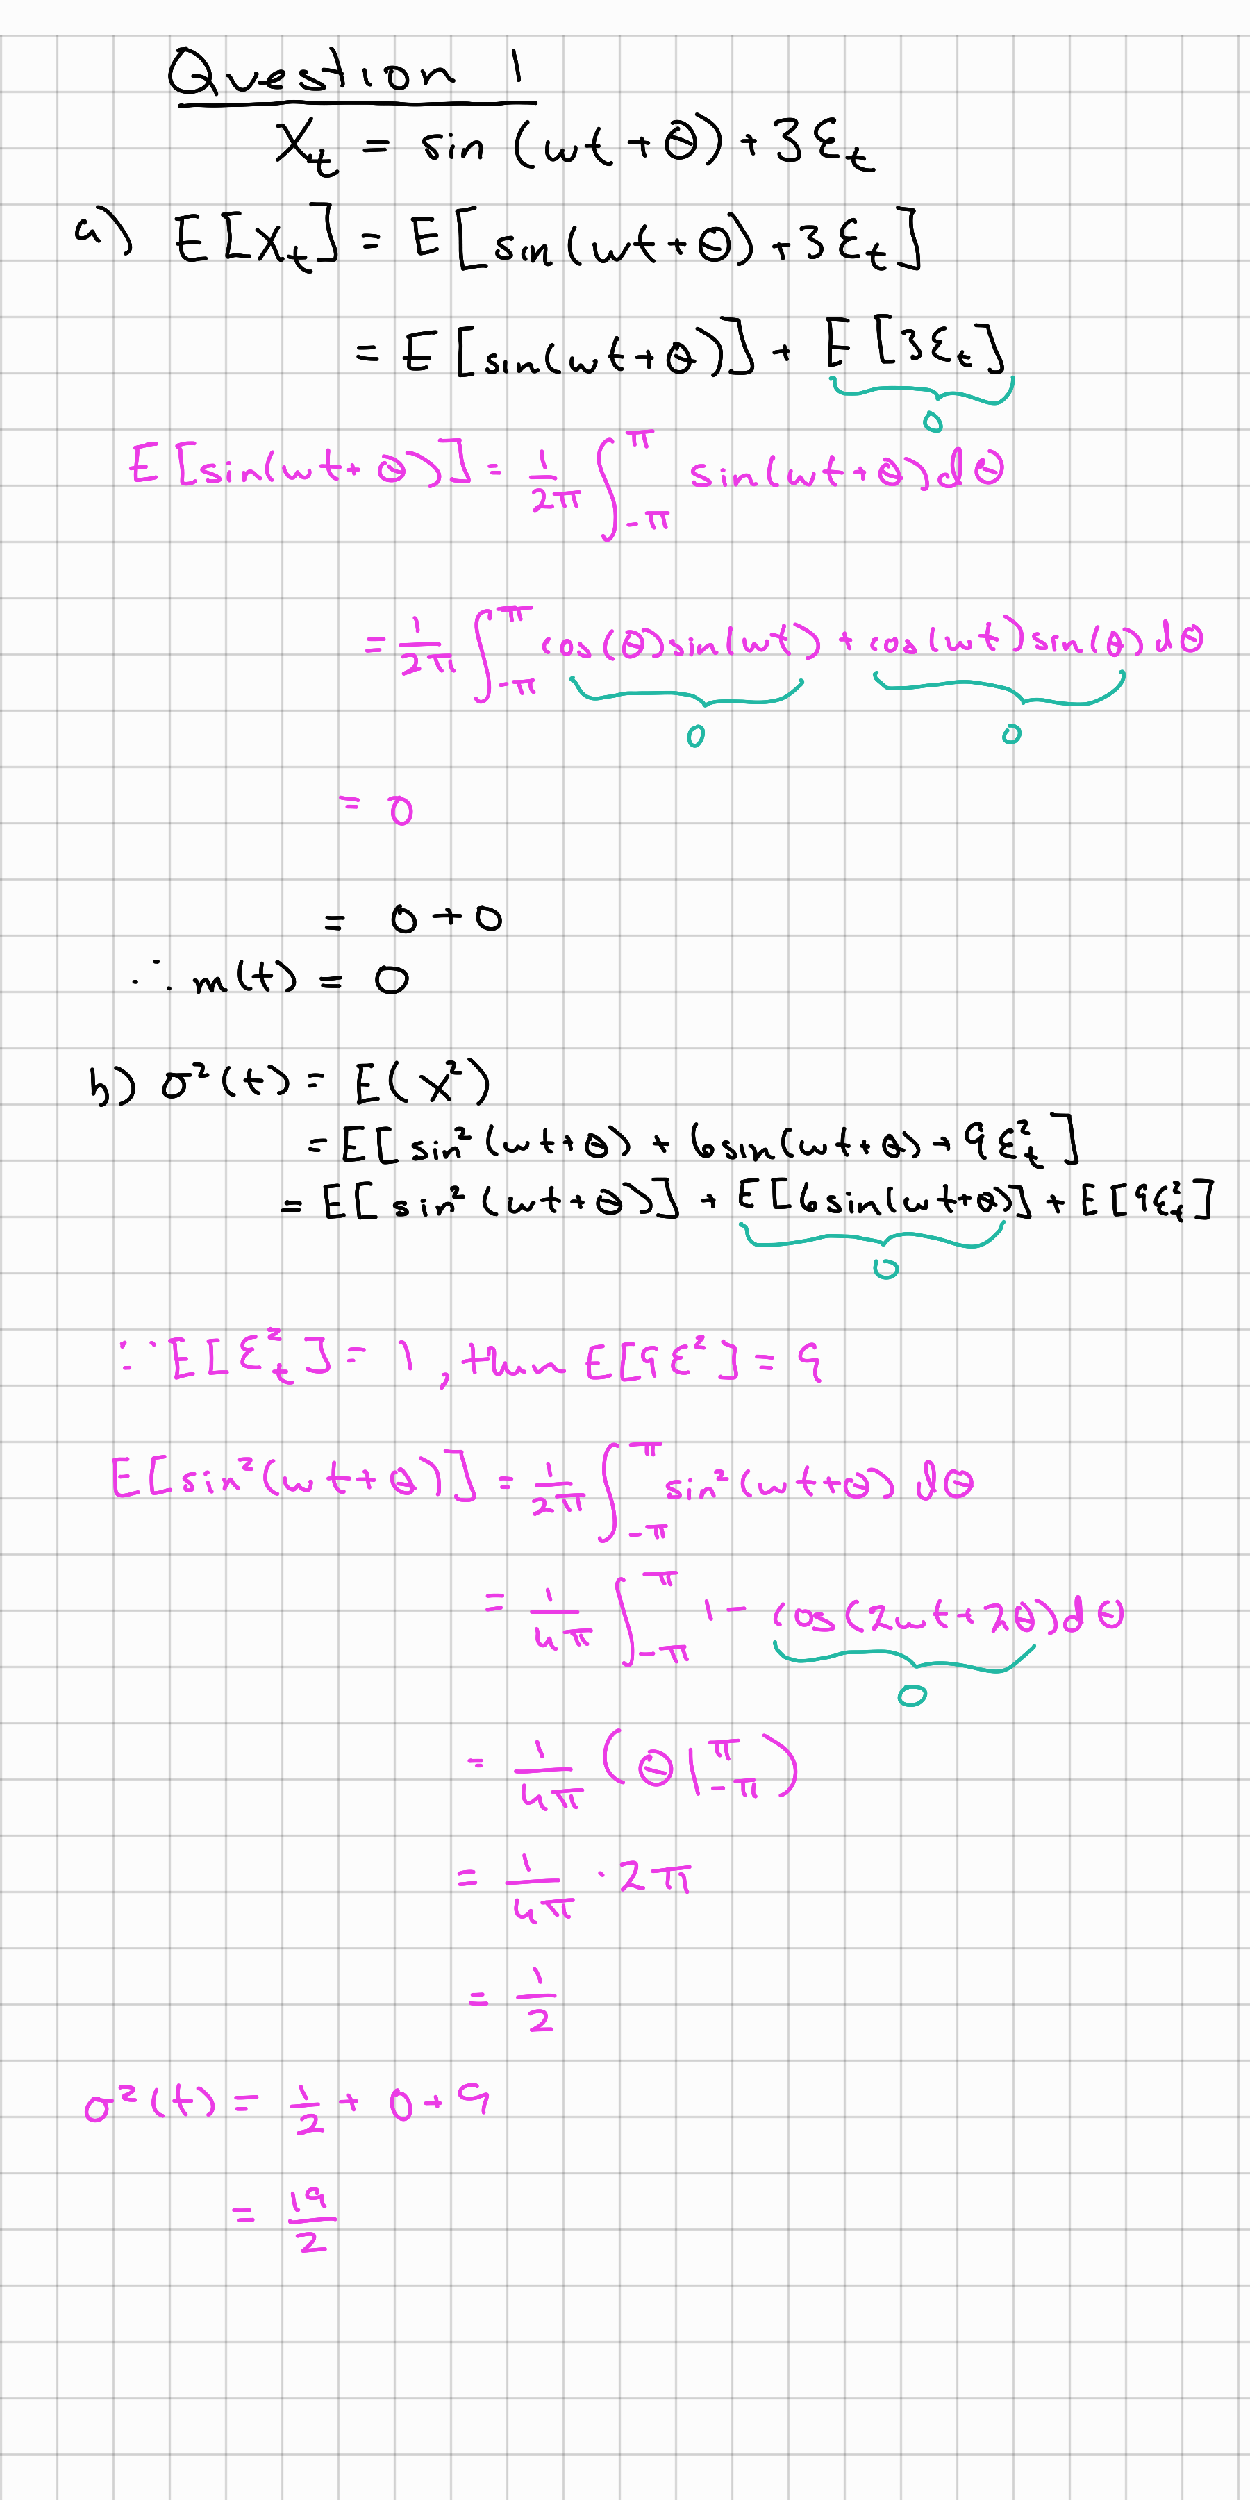
\includepdf{q1_1}
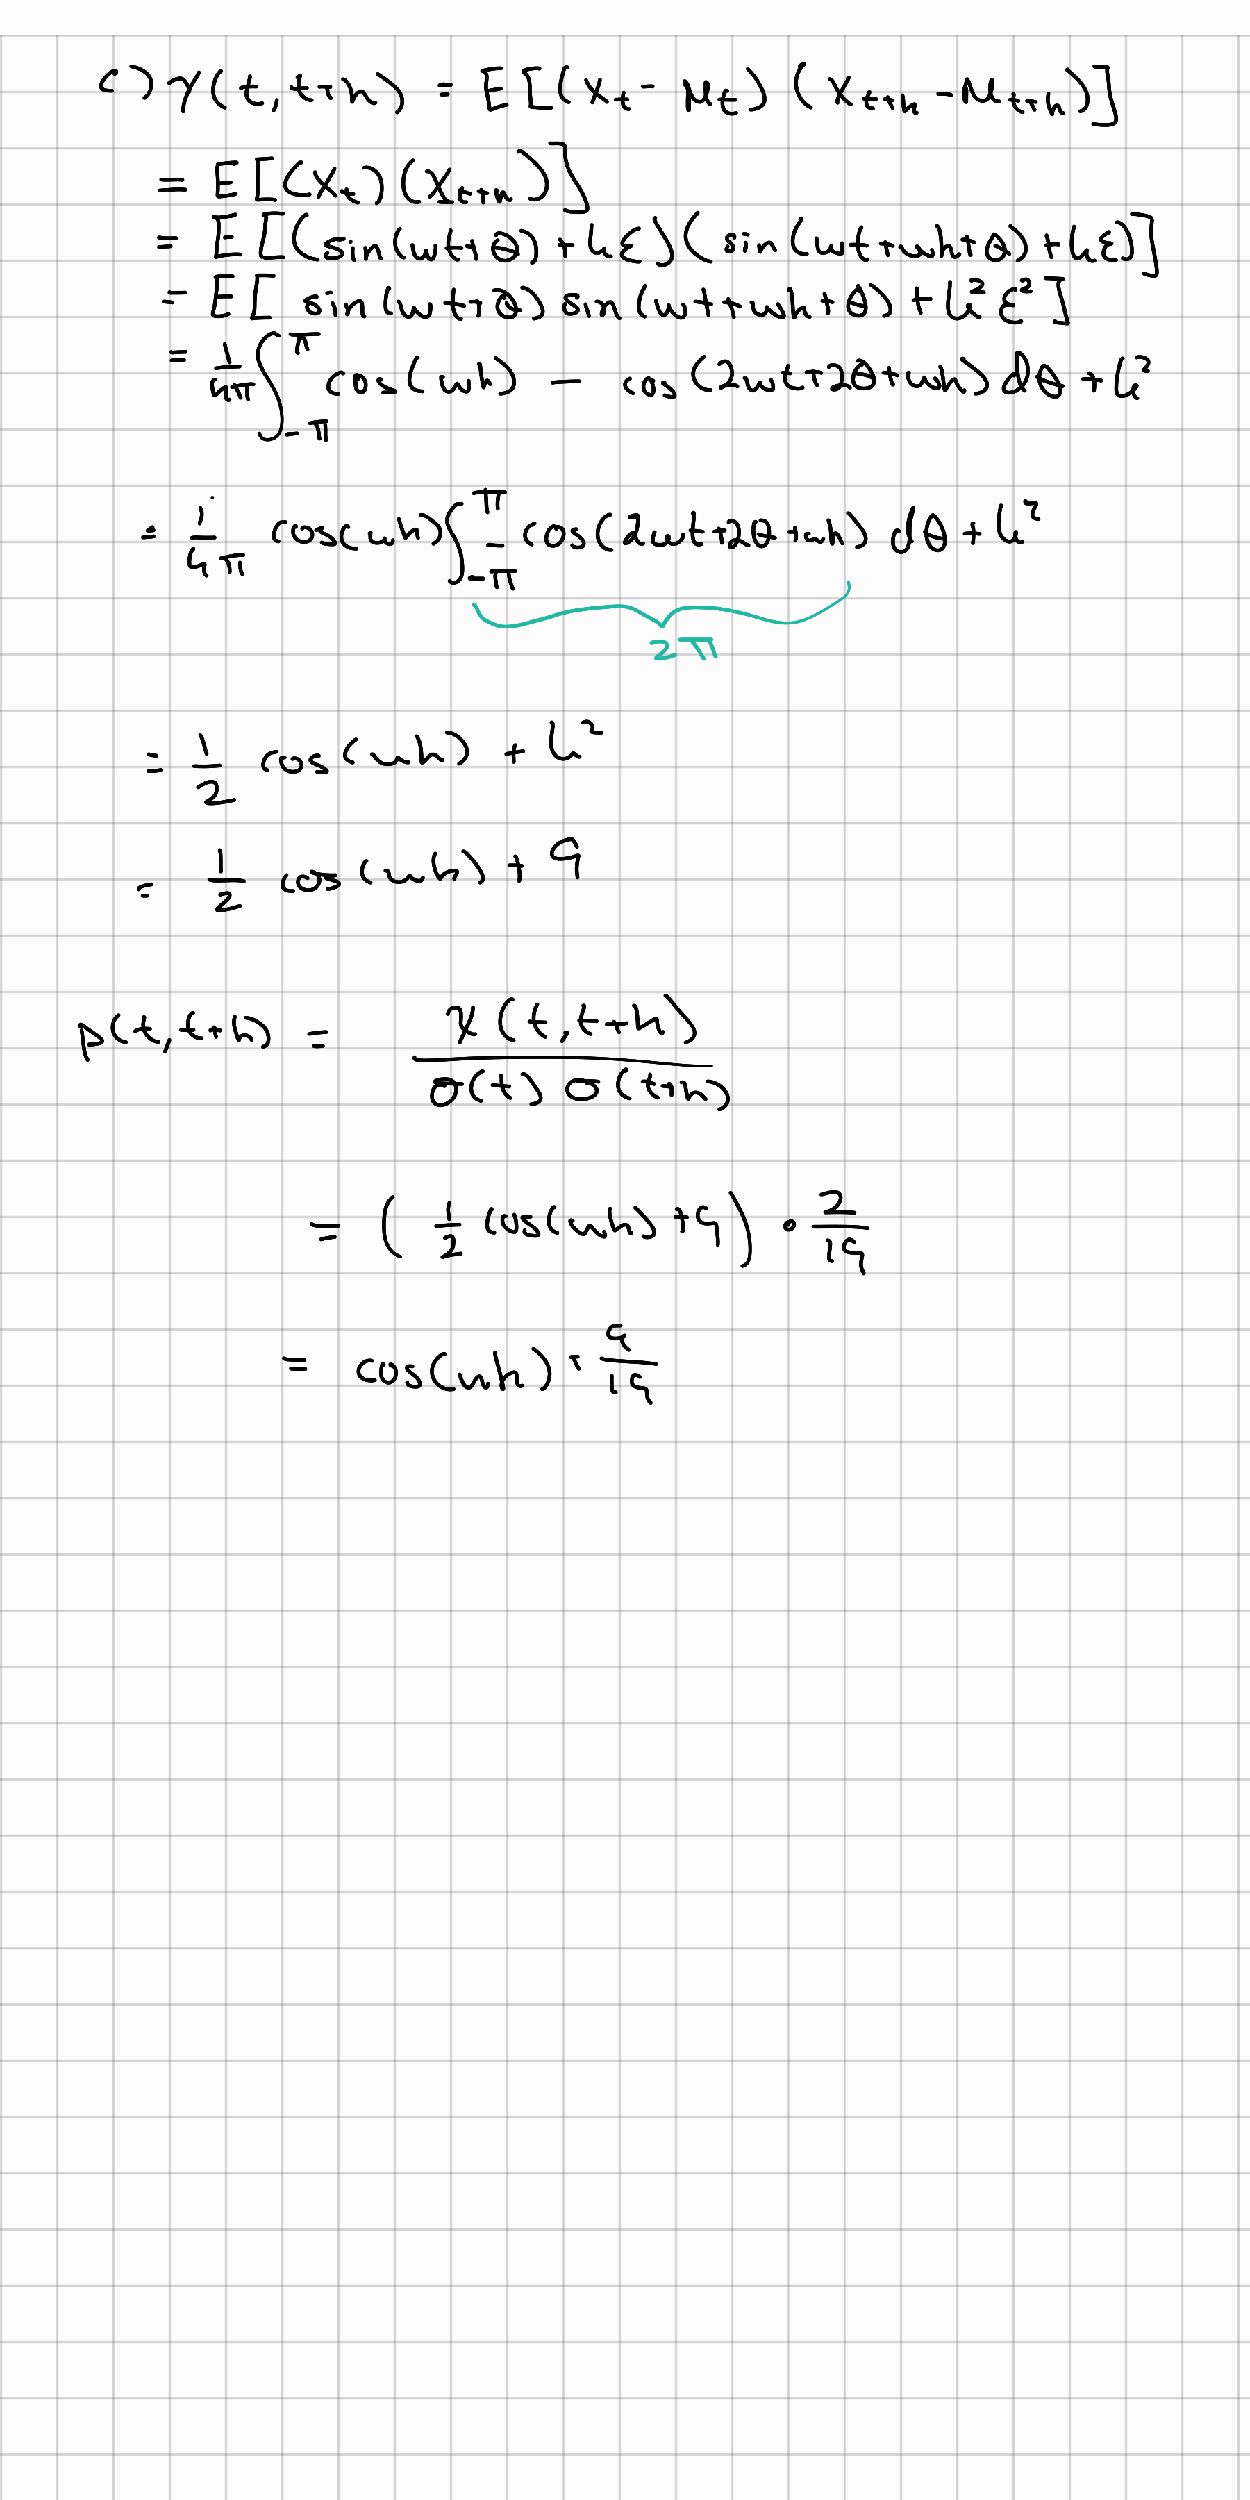
\includepdf{q1_2}
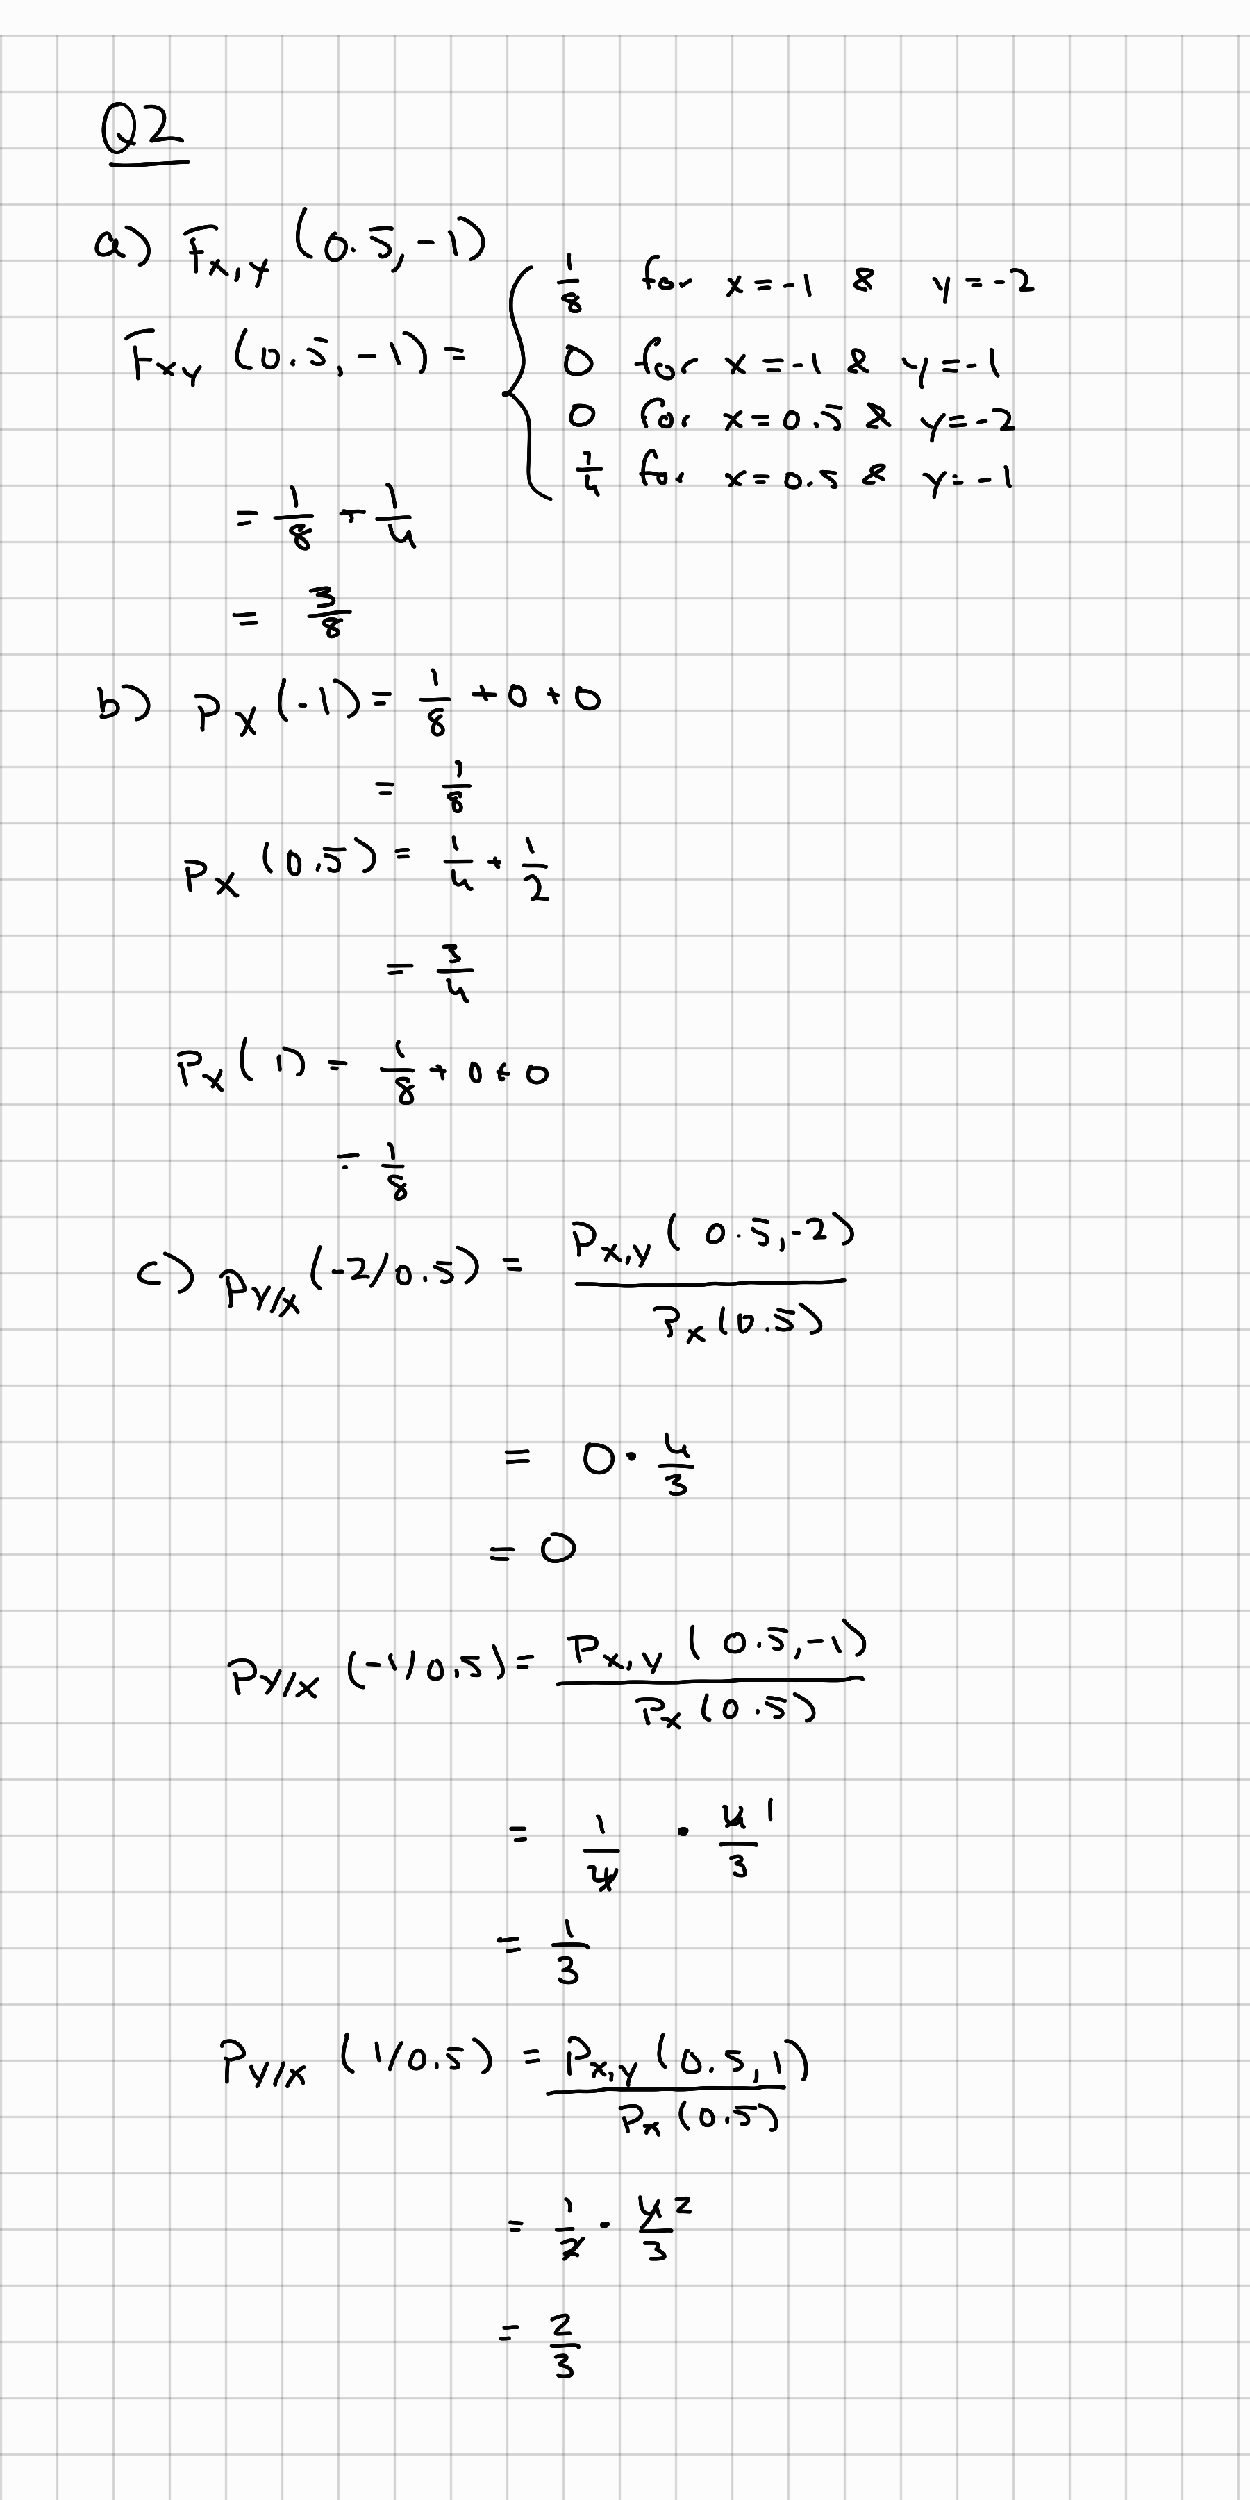
\includepdf{q2_1}
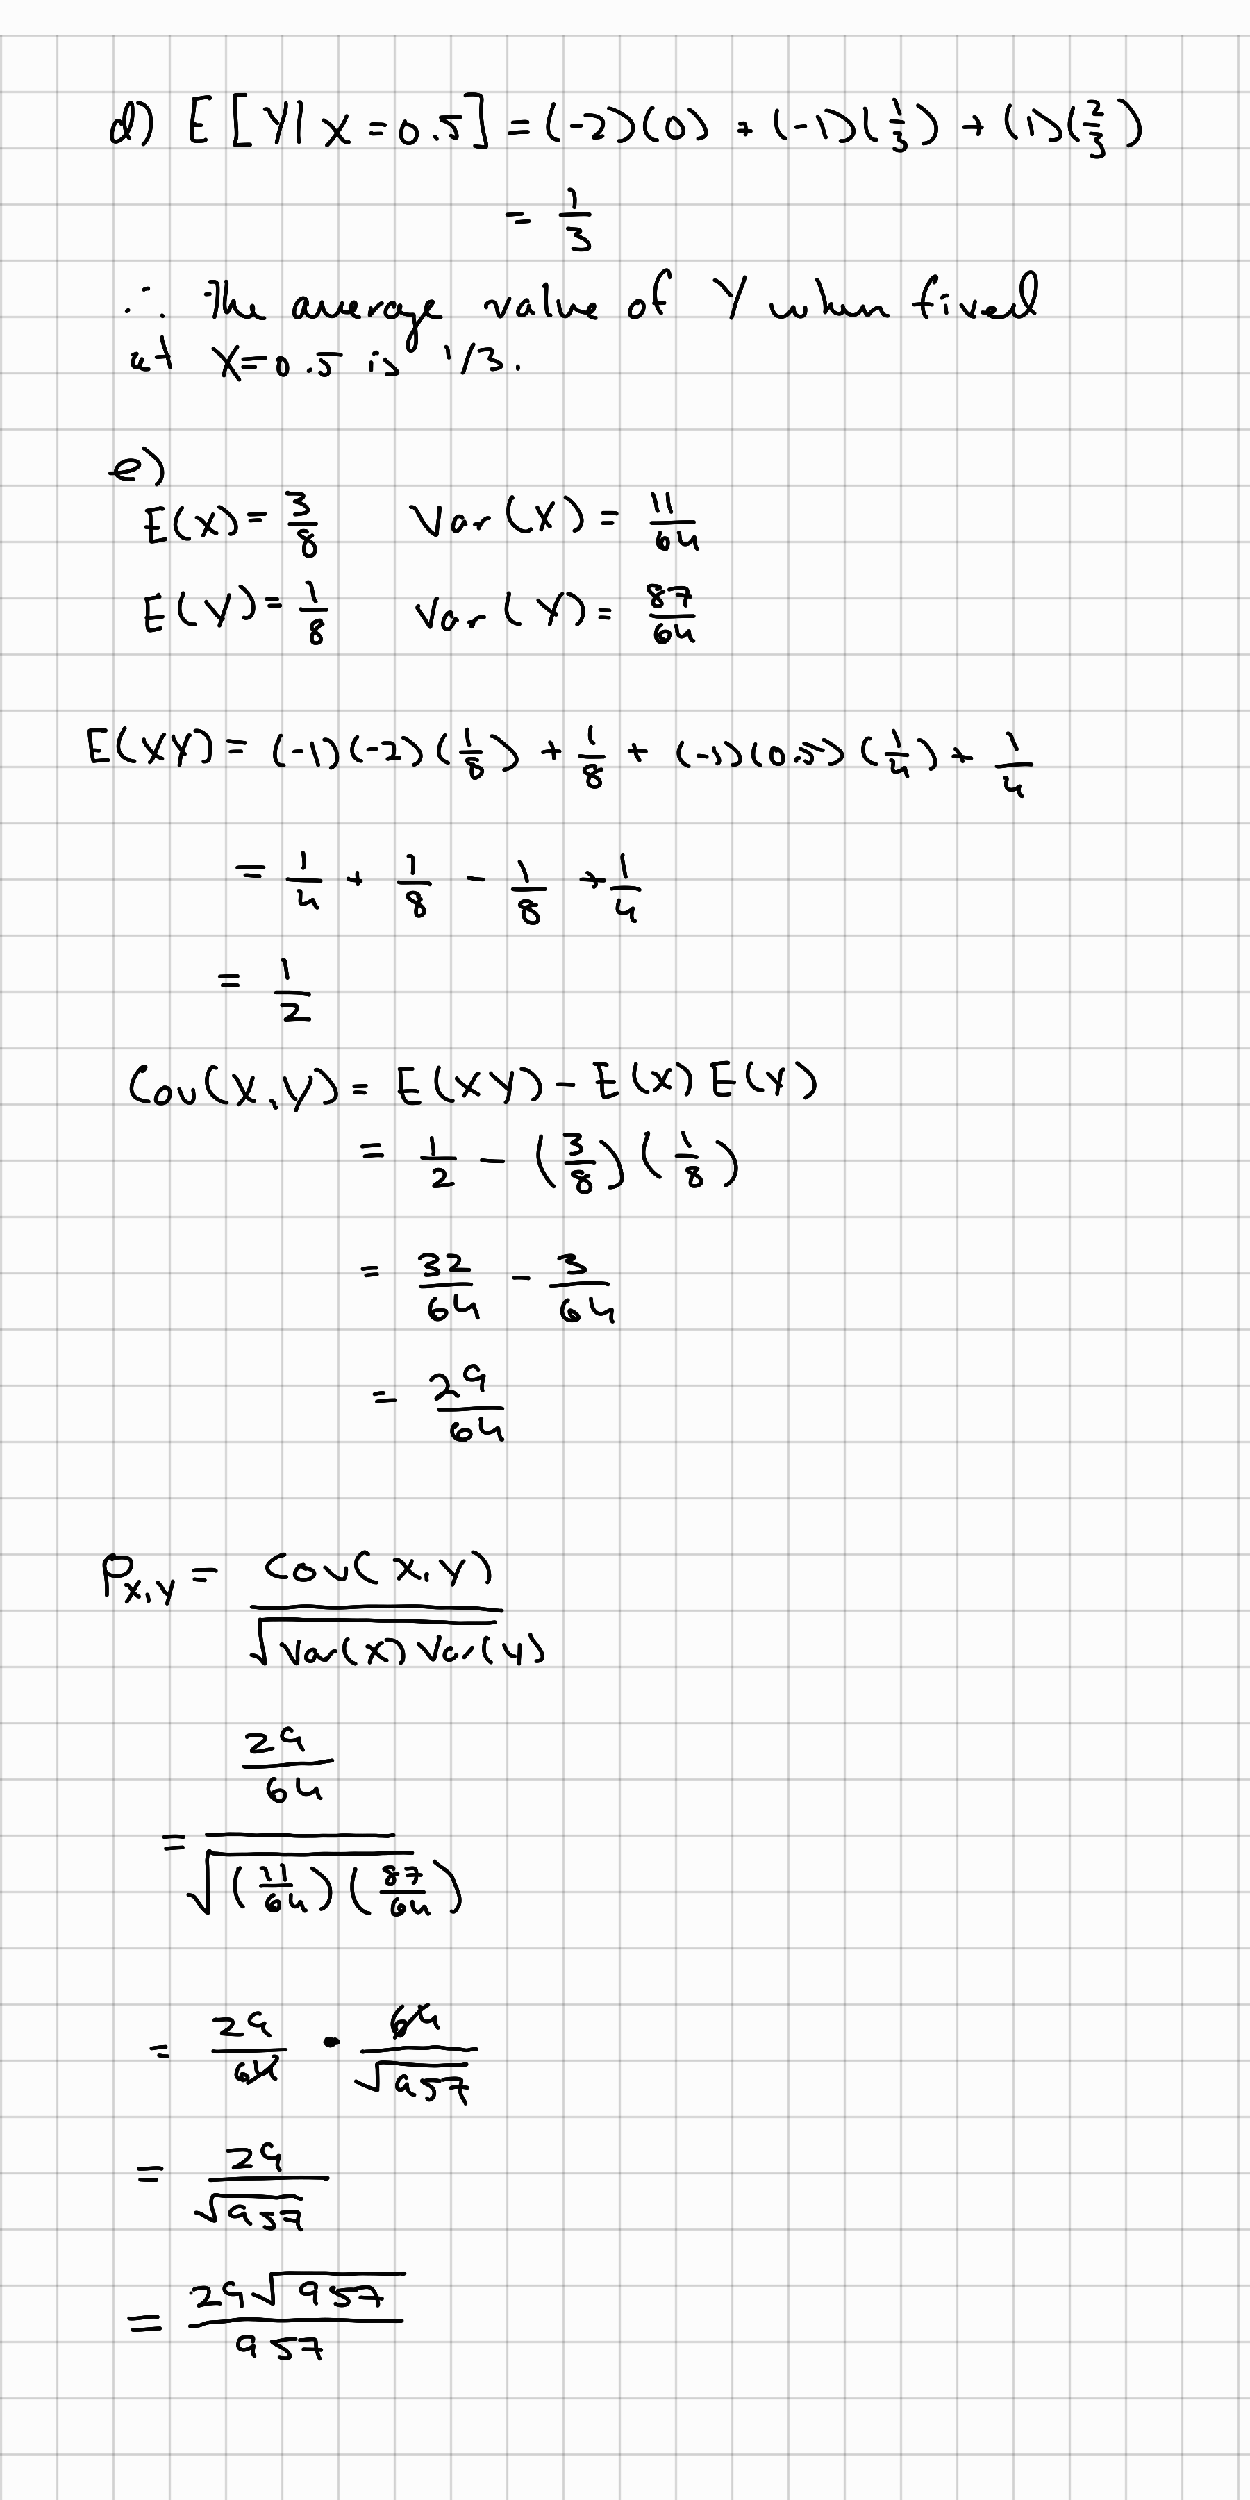
\includepdf{q2_2}
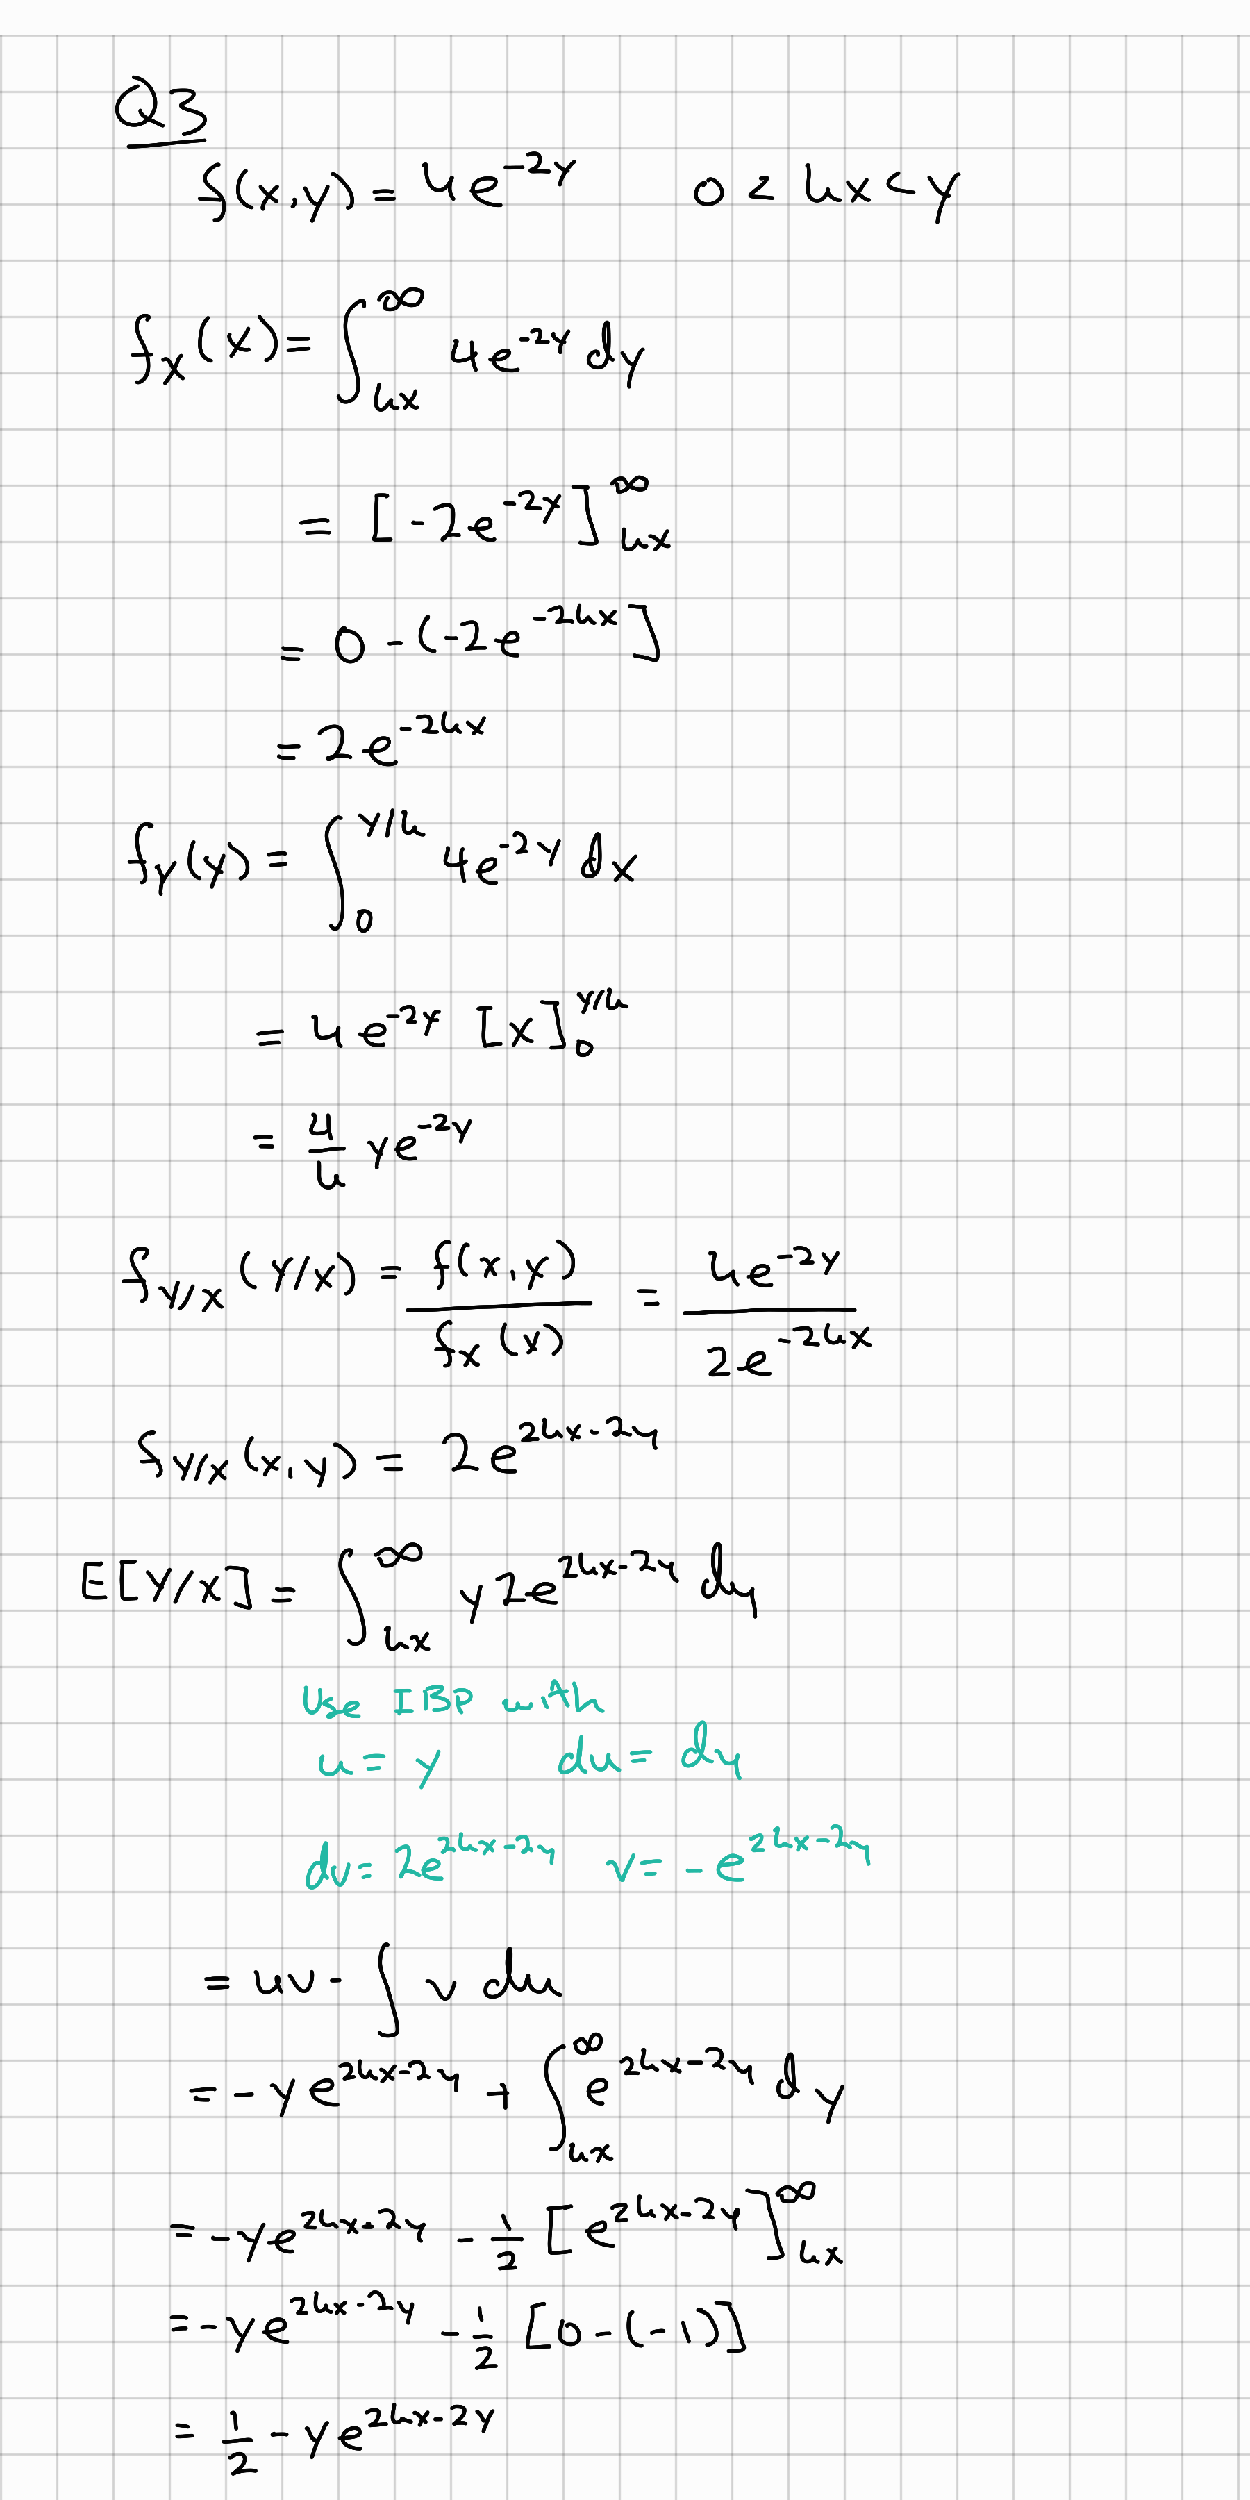
\includepdf{q3}

\newpage
\section*{Question 4}
\subsection*{A)}
To simulate a moving average process with $\theta = \cfrac{k}{10}$ driven by a
Gaussian
white noise, I created the R code \verb|q4a.r| where defined our parameters,
\verb|n| to define the number
of observations which I set to $1000$, \verb|theta| which is set to $0.3$ since
$k=3$. Lastly as defined
in the question, we set the variable \verb|sigma| to $1$. To generate the
Gaussian white noise, I use the
\verb|rnorm| function which uses the normal distribution and is randomized to
simulate the white noise. To intialize
the moving average process, we use the \verb|rep| function which replicates
elements of a list, we set this from $0$ to \verb|n|.
After we create a loop to define each \verb|t| in the moving average process
using the formula given. After
we plot our function.

\begin{file}[q4a.r]
	\lstinputlisting[language=r]{code/q4a.r}
\end{file}
\begin{center}
	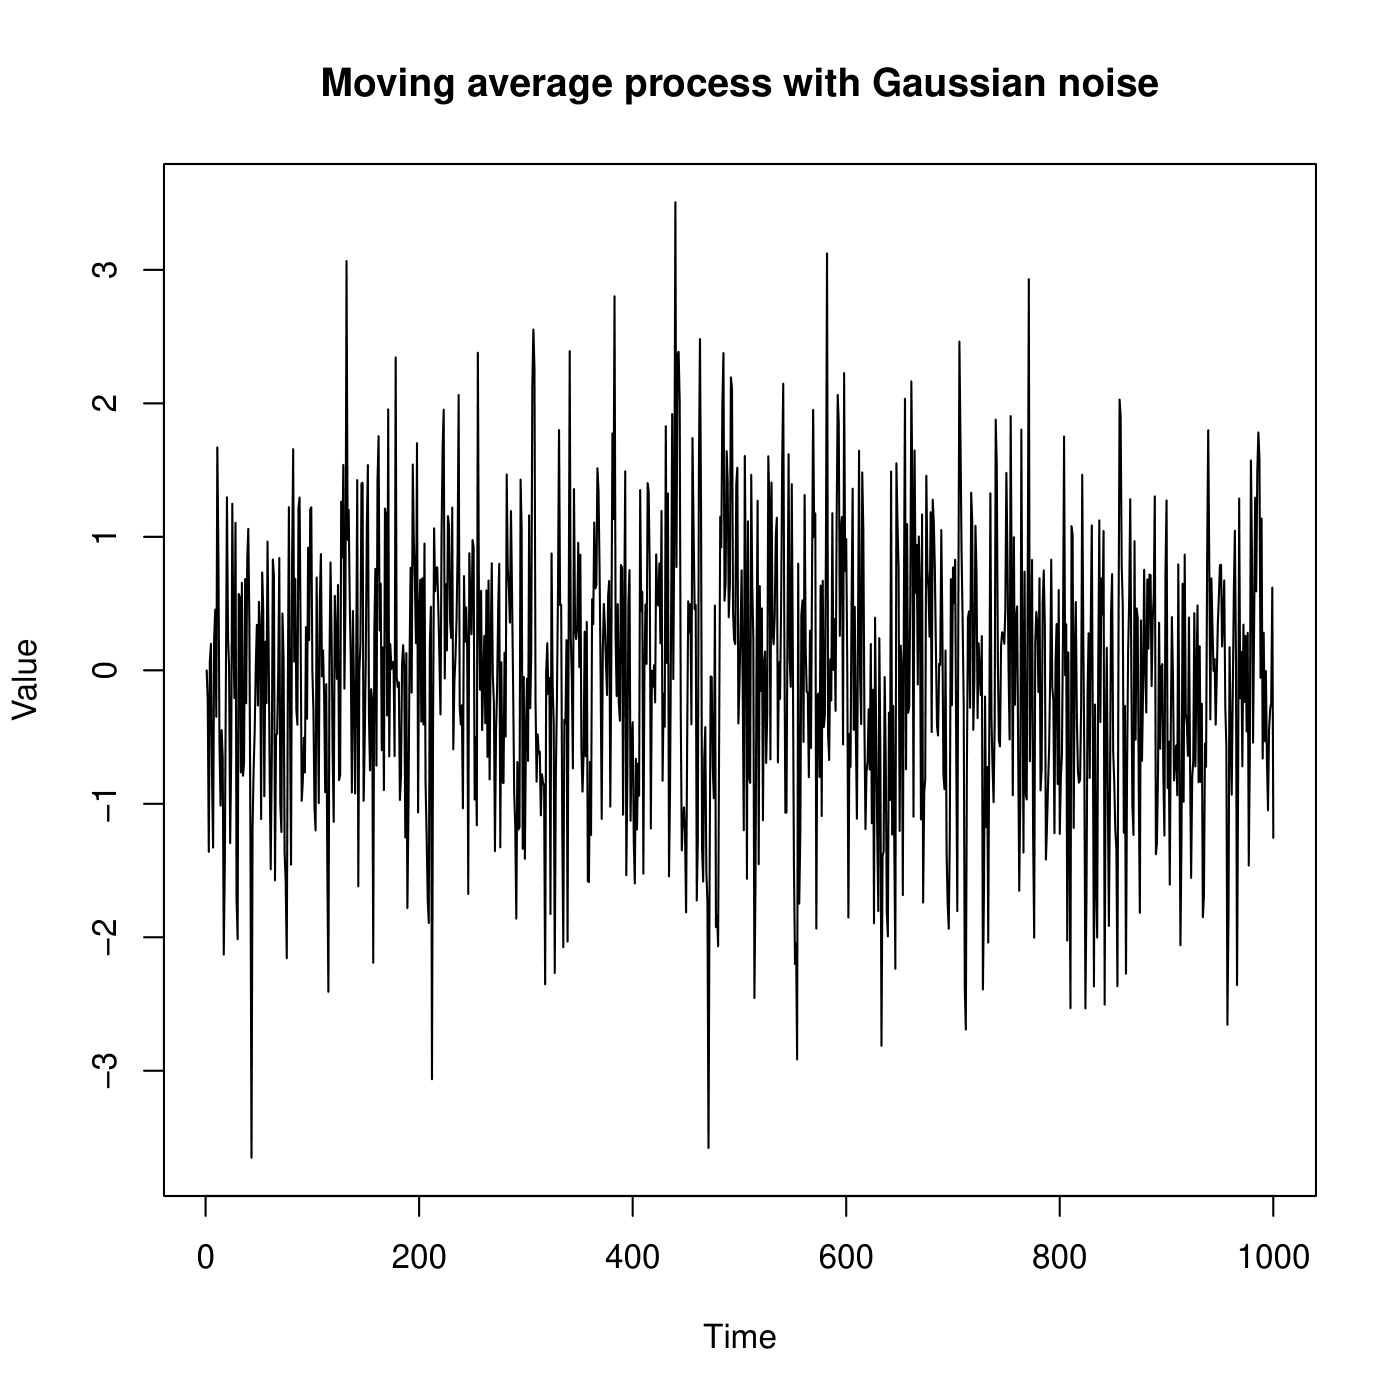
\includegraphics[scale=0.47]{code/q4a}
\end{center}

\subsection*{B)}
To simulate the moving average process with t-distribution with 4 degrees of
freedom, we will set similar
parameters like A), with $n=1000$, $theta = 0.3$, and $df=4$, After to generate
the randomized t-distribution,
we will use the \verb|rt| function with \verb|n| and \verb|df=df|. After we
will intialize and define the moving
average process like we had done before, and after we will plot our simulated
values.

\begin{file}[q4b.r]
	\lstinputlisting[language=r]{code/q4b.r}
\end{file}

\begin{center}
	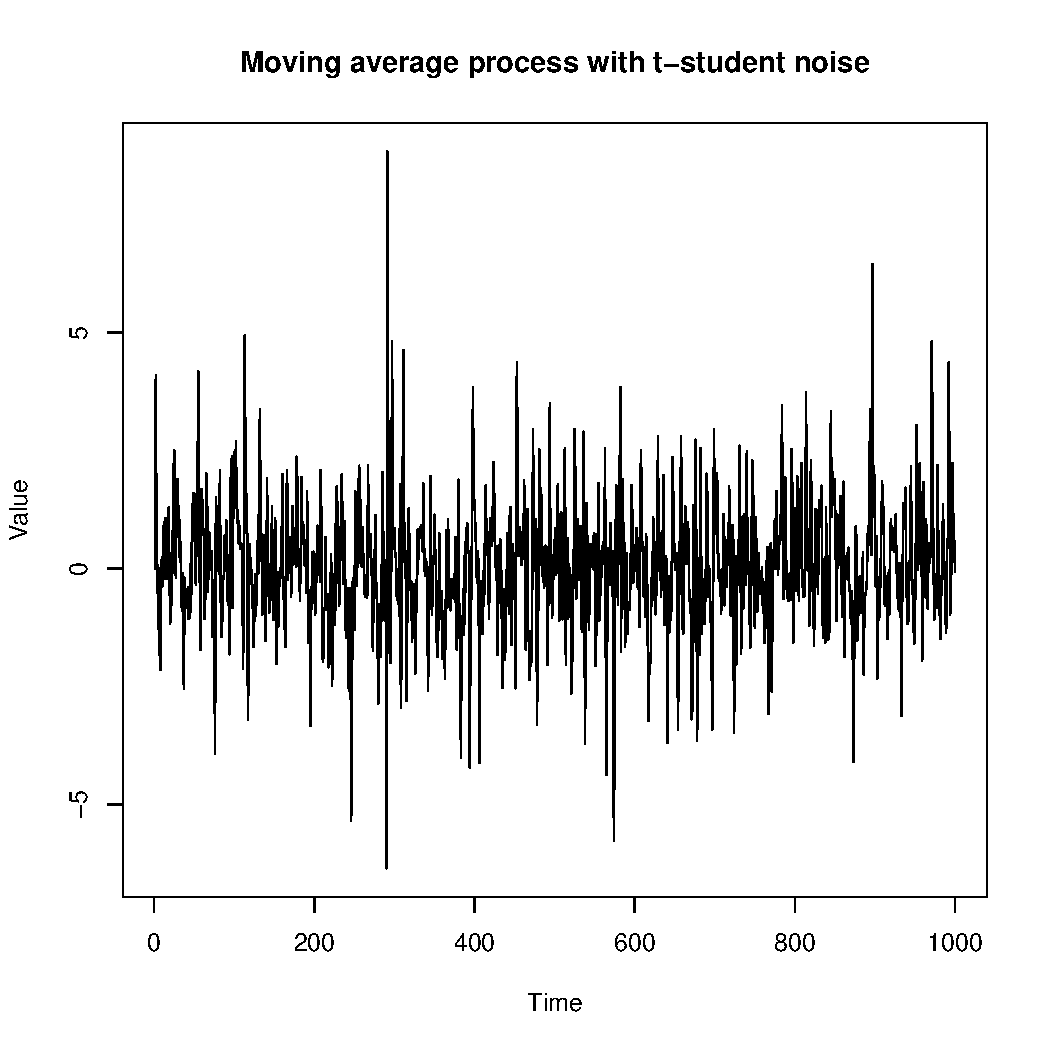
\includegraphics[scale=0.47]{code/q4b}
\end{center}
\newpage
\subsection*{C)}

\begin{file}[q4c.r]
	\lstinputlisting[language=r]{code/q4c.r}
\end{file}

The provided R code sets up a moving average process of order $1$ with Gaussian
noise, calculates the empirical autocorrelation of the process at different
lags, and plots the autocorrelation function. The
empirical autocorrelation function is calculated as the ratio of the covariance
between the series at time $t$ and $t + h$ and the variance of the series. The
plot
shows the autocorrelation values for each lag from $0$ to $10$. The term $\rho
	X(1)$
represents the autocorrelation of the process at lag 1, indicating how much the
current value of the process depends on its previous value. For a moving
average process of order $1$.

\begin{center}
	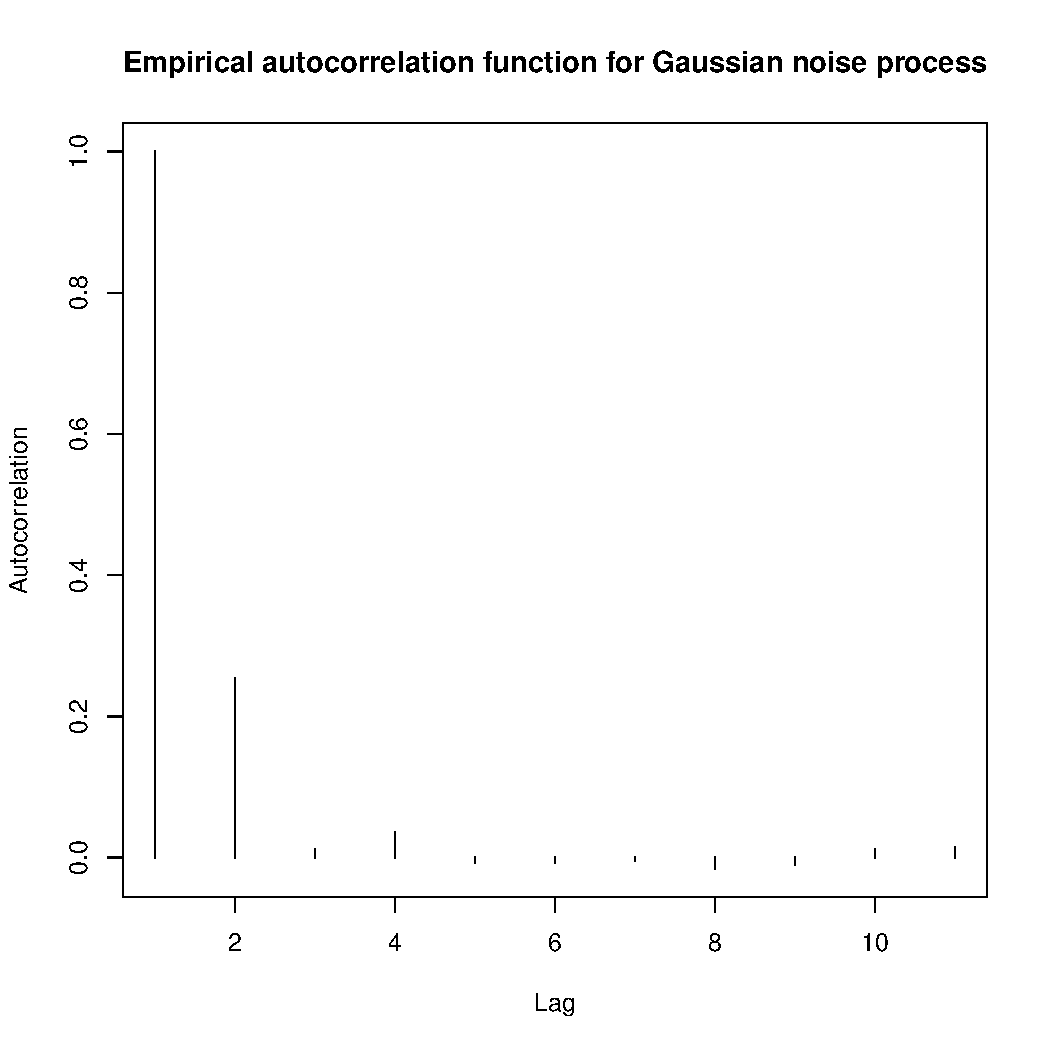
\includegraphics[scale=0.4]{code/q4c}
\end{center}

\section*{Question 5}

For question 5, I solved the problem by utilizing Python classes to handle
finding each subsection of this question
so I can present the final answers in a complete table. To answer each
subsection I will provide the snippet of the python
file \verb|q5.py| that corresponds with finding the said problem. At the end
once the code is shown, I will present the
results in a neat table. The reason I chose to use a Python class is because
all of the poisson files were identical,
which means I would be able to handle the repetitive tasks effectively.

\subsection*{i)}
First we need to be able to load the data and estimate our $\lambda$ value. To
begin in our code, we will be using the
\verb|pandas| library to read an excel file and use the second column which
contains the arrivals. We will need to be able
to calculate the poisson distribution, so we will need to make use of the
\verb|scipy| library, and lastly for better
numerical capabilities we will be using the \verb|numpy| library.

We will be creating a class called \verb|PoissonData| and to create a new
instance of it, we will define a constructor
which will take in a file name, we will read it use the first column which will
be assigned to the \verb|arrivals| field,
then we will take the mean of the arrivals and that will be our $\lambda$
estimate and used later we will set $\mu$ to 30.
This can all be seen below:

\begin{file}[q5.py i)]
	\lstinputlisting[linerange={1-10},language=python]{code/q5.py}
\end{file}

\subsection*{ii)}

To calculate the probability of  arrivals that occur in the interval of 5
hours, we will first calculate the rate
which is found by $\lambda * \frac{5}{24}$ then to get the probability we use
the Poisson PMF from $0$ to our rate.
This is all calculated in our function \verb|no_arrivals_5_hours_prob| in the
\verb|PoissonData| class:

\begin{file}[q5.py ii)]
	\lstinputlisting[language=python, linerange={11-14}]{code/q5.py}
\end{file}

\subsection*{iii)}
To calculate the probability of at least one arrival occurs, we will be needing
to find $1-Poisson(0,\lambda)$ as
shown in the function \verb|at_least_one_arrival_prob| in the
\verb|PoissonData| class:

\begin{file}[q5.py iii)]
	\lstinputlisting[language=python, linerange={15-18}]{code/q5.py}
\end{file}

\subsection*{iv)}
To calculate the mean and variance of the arrival in a day, we need to remember
that in a Poisson distribution,
$E(X) = \lambda$ and $Var(X) = \lambda$, so in our \verb|mean_arrivals| and
\verb|variance_arrivals| functions, we
return our \verb|lambdaHat| field.

\begin{file}[q5.py]
	\lstinputlisting[language=python, linerange={19-24}]{code/q5.py}
\end{file}

\subsection*{v)}
To calculate the average and standard deviation of the total time it takes
for a patient in a single day using $\mu = 30$ is by multiplying \verb|self.mu|
by the mean
of arrivals and standard deviation respectively. This can be seen below:

\begin{file}[q5.py]
	\lstinputlisting[language=python, linerange={25-30}]{code/q5.py}
\end{file}

\subsection*{Results}
To get the results for each file, I did add an extra method to turn our results
into strings where each
result from i)\dots v) would be rounded to 4 decimal points. I created a
\verb|results.txt| file where each of the results
were appended and in a \verb|for| loop all files from $0\dots 9$ were
calculated.

\begin{file}[q5.py]
	\lstinputlisting[language=python, linerange={31-58}]{code/q5.py}
\end{file}

Instead of showing a $100$ line text file, I opted to neatly format it into a
table where we get our
results for each file:

\begin{table}[h]
	\centering
	\small
	\begin{tabular}{|l|c|c|c|c|c|c|c|}
		\hline
		File    & $\lambda$ & Prob. No 5 Hrs   & Prob. At Least One &
		Mean    & Variance  & Avg. Time (mins) & Std. Dev. (mins)
		\\
		\hline
		poissn0 & 3.0606    & 0.5285           & 0.9531             &
		3.0606  & 3.0606    & 91.8182
		        & 58.4208
		\\
		poissn1 & 2.9596    & 0.5398           & 0.9482             &
		2.9596  & 2.9596    & 88.7879
		        & 49.5958
		\\
		poissn2 & 2.9293    & 0.5432           & 0.9466             &
		2.9293  & 2.9293    & 87.8788
		        & 42.4810
		\\
		poissn3 & 2.9394    & 0.5421           & 0.9471             &
		2.9394  & 2.9394    & 88.1818
		        & 54.1797
		\\
		poissn4 & 3.1111    & 0.5230           & 0.9554             &
		3.1111  & 3.1111    & 93.3333
		        & 47.5094
		\\
		poissn5 & 3.2121    & 0.5121           & 0.9597             &
		3.2121  & 3.2121    & 96.3636
		        & 54.5941
		\\
		poissn6 & 3.1515    & 0.5186           & 0.9572             &
		3.1515  & 3.1515    & 94.5455
		        & 51.8489
		\\
		poissn7 & 3.0000    & 0.5353           & 0.9502             &
		3.0000  & 3.0000    & 90.0000
		        & 50.1630
		\\
		poissn8 & 3.3131    & 0.5015           & 0.9636             &
		3.3131  & 3.3131    & 99.3939
		        & 52.0757
		\\
		poissn9 & 3.2121    & 0.5121           & 0.9597             &
		3.2121  & 3.2121    & 96.3636
		        & 51.1192
		\\
		\hline
	\end{tabular}
	\caption{Poisson Data Results}
\end{table}

\section*{Question 6}
The timeseries data we will be analyzing is the Apple stock price found in
\verb|AAPL.csv|, to solve each
part we will be using R in the file \verb|q6.r|.
\subsection*{i)}
To plot the Apple time series we will need to read the \verb|csv| file, get the
daily returns from the \verb|Change| column,
then we need to convert each of the strings into numerical numbers, we also get
the stock prices from the \verb|Price| column.
With the \verb|daily_returns| and \verb|prices| variables, we will create a
dataframe with the daily returns as the x-axis
and prices as the y-axis. Lastly we plot the prices as a scatterplot:

\begin{file}[q6.r i)]
	\lstinputlisting[language=r, linerange={1-24}]{code/q6.r}
\end{file}

\begin{figure}[h!]
	\centering
	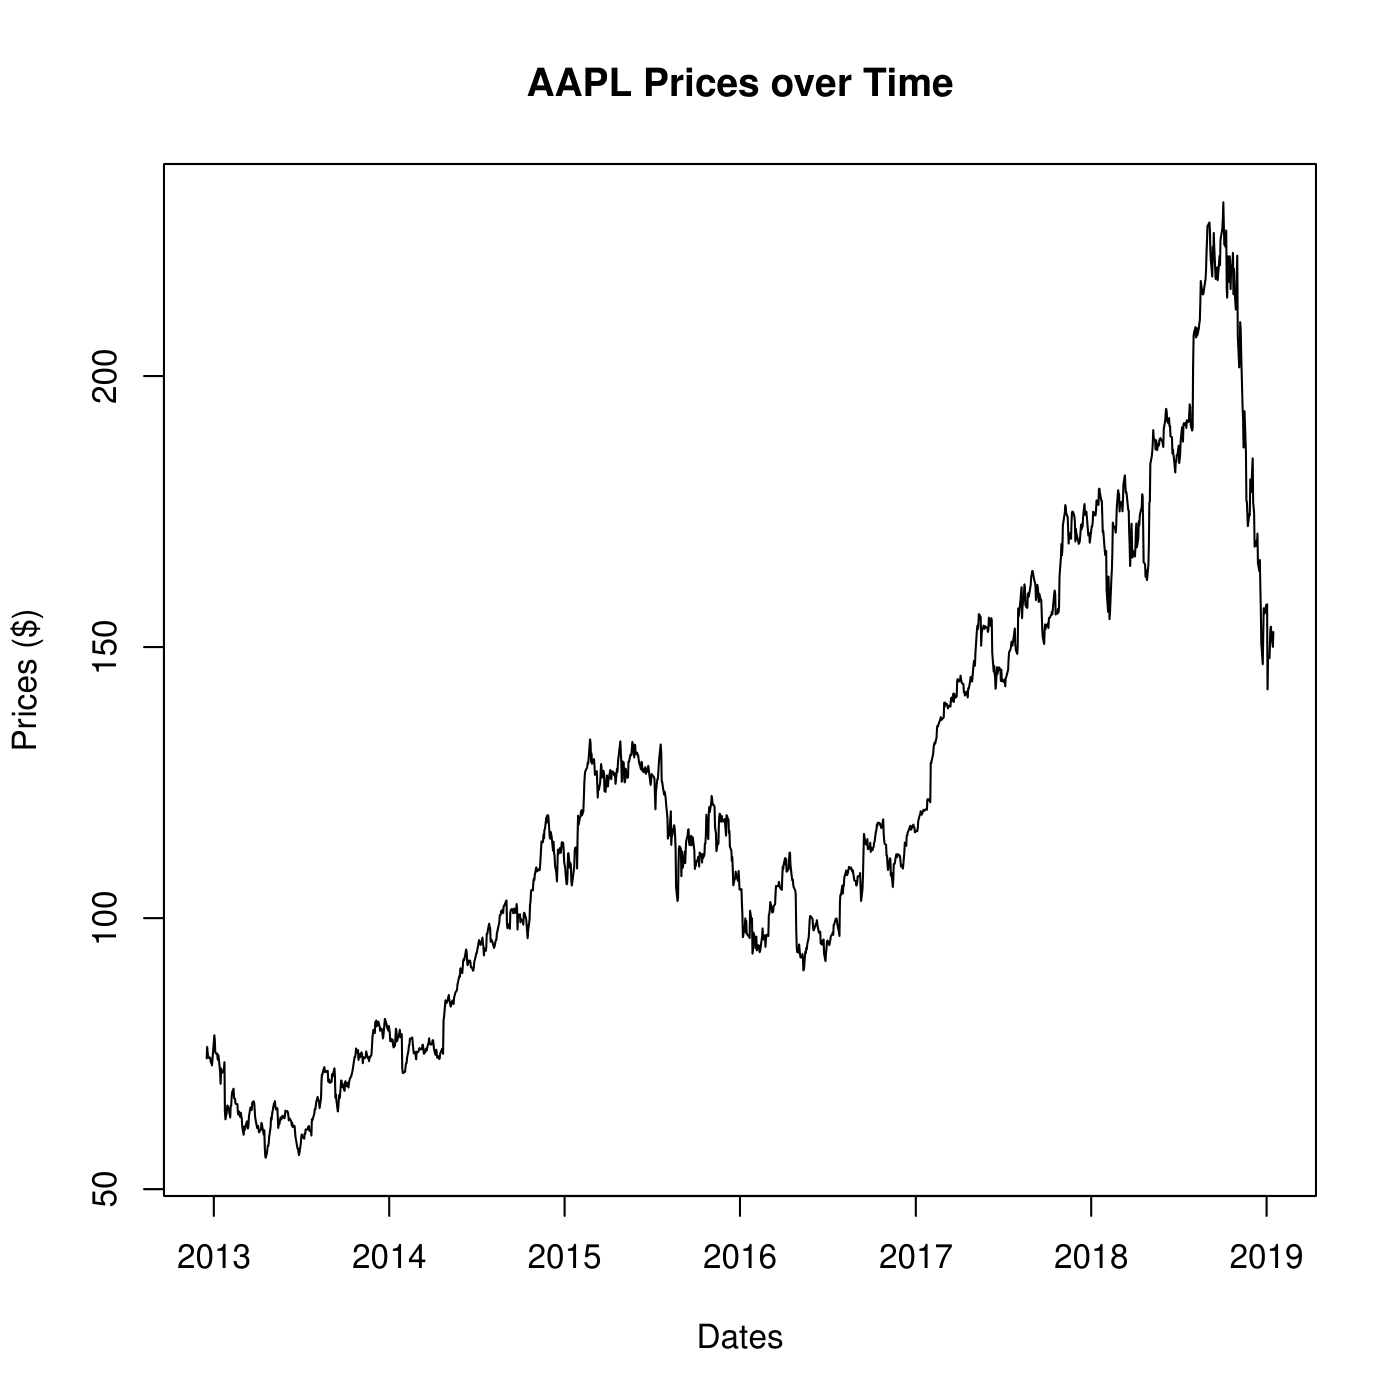
\includegraphics[scale=0.55]{code/q6-1.png}
\end{figure}

\subsection*{ii)}
To calculate the first four moments (mean, standard deviation, skewness and
kurtosis) for the prices,
and daily returns, we will need to use the functions \verb|mean|, \verb|sd|,
\verb|skewness| and \verb|kurtosis|
respectively for the variables \verb|prices| and \verb|dailyReturns| that were
calculated previously.

\begin{file}[q6.r ii)]
	\lstinputlisting[language=r, linerange={25-45}]{code/q6.r}
\end{file}

\noindent When we run our script we get the following result:

\begin{verbatim}
Mean of prices: 120.4879 
Standard deviation of prices: 41.64585 
Skewness of prices: 0.5805278 
Kurtosis of prices: 2.611525 

Mean of daily returns: 0.06097975 
Standard deviation of daily returns: 1.58414 
Skewness of daily returns: -0.4705426 
Kurtosis of daily returns: 8.834479 
\end{verbatim}

\end{document}